
\chapter{The equations of fluid dynamics}\label{chap1}


\section{Introduction}\label{chap1:sec1.1}

In\pageoriginale this section we merely write down the basic equations
of fluid dynamics involving one space variable and time. (This occurs,
for instance, in the study of the flow of a gas in a narrow
cylindrical tube where the state of flow is constant across any cross
section and so depends only on the linear coordinate measured along
the axis of the tube, and on time). From these general equations, we
write down three simple particular equations whose properties will
then be studied in the sequel. We will return to the general equations
in section \ref{chap9}.

\section{Notations}\label{chap1:sec1.2}

To start with we put down the various notations which will be used in
writing these equations. We will denote by $\rho$, the density of
the fluid; by $V = \dfrac{1}{\rho}$, the specific volume; by $p$,
the pressure; by $q$, the pseudo-viscosity term; by $\varepsilon$, the
internal energy per unit of mass; by $E$, the total energy per unit of
mass; by $u$, the velocity of the fluid; by $T$ the absolute
temperature.

One has the relation
\begin{equation*}
E = \varepsilon + \frac{1}{2} u^2\tag{1.1}\label{eq1.1}
\end{equation*}


We denote by $\mu$, the coefficient of viscosity and by $k$, the
coefficient of conductivity of the relevant fluid,

The quantities $\rho, p, \varepsilon$ and $T$ are thermodynamical
quantities and they are related by the {\em equations of state:}
\begin{equation*}
\left.
\begin{aligned}
p & = p \; (\rho, T)\\[3pt]
\varepsilon & = \varepsilon \; (\rho, T)
\end{aligned} \right\}
 \tag{1.2}\label{eq1.2}
\end{equation*}
For instance, in the case of a perfect fluid the equations (\ref{eq1.2})
assume the form 
\begin{equation*}
\left.
\begin{aligned}
p & = R \; \rho \; T \\[3pt]
 & = \dfrac{RT}{\gamma -1} 
\end{aligned} \right\}
 \tag{1.3}\label{eq1.3}
\end{equation*}\pageoriginale
where $R$ is the universal gas constant and $\gamma$ the constant
ratio of specific heats.

\section{Coordinate systems}\label{chap1:sec1.3}

In writing down the equations of fluid dynamics we express in
mathematical form the following three laws: the law of conservation of
mass, the law of conservation of quantity of movement (i.e. momentum)
and the law of conservation of energy.

One way write these equations in several equivalent forms. Chiefly,
one uses the two types of coordinate systems described below.
\begin{itemize}
\item[{\rm {\bf(i)}}] {\bf The Eulerian System.} Here the independent
  variables are $x$ and $t$, where $t$ is the time and $x$ is the
  position of a point in space with reference to a frame fixed in the
  laboratory. 

\item[{\rm {\bf(ii)}}] {\bf The Lagrangian System.} We now have the
  independent variables $a$ and $t$ where $t$ is as in (i). Now $a$ is
  the position at time $t = 0$, of the particle which is at position
  $x = x(a,t)$ at time $t$.
\end{itemize}

One assumes that the particles do not cross one another at any
instant. In other words, for every $t$, the transformation $a \mapsto
x(a,t)$ is invertible. If  we denote by $J$ the Jacobian of the
transformation, i.e.
\begin{equation*}
J = \frac{\partial x}{ \partial a}. \tag{1.4}\label{eq1.4}
\end{equation*}
then $J \neq 0$ everywhere.

Given any physical quantity in one system we can always express it in
the other using this transformation. Thus we have 
\begin{equation*}
f(x,t) = f(x(a,t),t) = f(a,t). \tag{1.5}\label{eq1.5}
\end{equation*}\pageoriginale 
The derivative of $\bar{f}$ w.r.t $t$ is given in terms of the
derivatives of $f$ by the relation 
\begin{equation*}
\frac{\partial \bar{f}}{\partial t} = \frac{\partial t}{\partial t} +
u \frac{\partial f}{\partial x} \tag{1.6}\label{eq1.6}
\end{equation*}
where $u$, the derivative of $x$ w.r.t. $t$, is the velocity of the
fluid particle at time $t$ which is at position $x$. The relation
(\ref{eq1.6}) leads to the following 

\begin{Definition}\label{chap1:def1.1}
The Lagrangian (or particular) time derivative of a function $f(x,t)$
is given by
\begin{equation*}
\frac{Df}{Dt} = \frac{\partial f}{\partial t} + u \frac{\partial
  f}{\partial x} \tag{1.7}\label{eq1.7}
\end{equation*}
\end{Definition}

\section{The equations in eulerian system}\label{chap1:sec1.4}

We now write down the equations of fluid dynamics in Eulerian form, in
the slab symmetric case. The equations of one-dimensional cylindrical
or spherical symmetric flows will assume different forms. The
derivations of these equations can be found in any standard text on
fluid dynamics.

\medskip
\noindent{\textbf{E1. Conservation of Mass}}
\begin{equation*}
\frac{\partial \rho}{\partial t} + \frac{\partial}{\partial x}
(\rho u) = 0 \tag{1.8}\label{eq1.8}
\end{equation*}

\medskip
\noindent{\textbf{E2. Conservation of Momentum}}
\begin{equation*}
\frac{\partial}{\partial t} (\rho u)+ \frac{\partial}{\partial x}
\left(\rho u^2 + p - \frac{4}{3} \mu \frac{\partial u}{\partial x}\right) = g
\rho \tag{1.9}\label{eq1.9}
 \end{equation*}
where $g$ is the volume acceleration applied from the exterior of the
system.

\medskip
\noindent{\textbf{E3. Conservation of Energy}}
\begin{equation*}
\frac{\partial}{\partial t} (\rho E) + \frac{\partial }{\partial x}
\left(\rho u E + pu - \frac{4}{3} \mu u \frac{\partial u}{\partial x}\right)
= \rho gu + \frac{\partial }{\partial x} \left(k \frac{\partial
  T}{\partial x}\right). \tag{1.10}\label{eq1.10}
\end{equation*}\pageoriginale

\begin{exercise}\label{chap1:exer1.1}
\begin{itemize}
\item[{\rm (a)}] Starting from (E1) and (E2) show that one can write
  (E2) also as 
\begin{equation*}
\frac{\partial u}{\partial t} + u \frac{\partial u}{\partial x} +
\frac{1}{\rho} \frac{\partial}{\partial x} \left(p -\frac{4}{3} \mu
\frac{\partial u}{\partial x}\right) = g. \tag*{(E2$'$)}
\end{equation*}

\item[{\rm (b)}] Using (E1) and (E2$'$) show that one can rewrite (E3)
  as 
\begin{equation*}
\frac{\partial}{\partial t} (\rho \varepsilon)
+\frac{\partial}{\partial x} (\rho u \varepsilon) + p
\frac{\partial u}{\partial x} - \frac{4}{3} \mu \left(\frac{\partial
  u}{\partial x}\right)^2 = \frac{\partial}{\partial x} \left(k  \frac{\partial
  T}{\partial x}\right) \tag*{E3$'$}
\end{equation*}
or as
\begin{equation*}
\frac{\partial \varepsilon}{\partial t} + u \frac{\partial
  \varepsilon}{\partial x} + \frac{1}{\rho} \left(p-\frac{4}{3} \mu
\frac{\partial u}{\partial x }\right) \frac{\partial u}{\partial x} =
\frac{1}{\rho} \frac{\partial}{\partial x} \left(k \frac{\partial
  T}{\partial x}\right). 
\tag*{E3$''$}
\end{equation*}
\end{itemize}
\end{exercise}

\begin{remark}\label{chap1:rem1.1}
Equations (E3$'$) and (E3$''$) give the law of conservation of energy
in terms of the {\em internal} energy while (E3) gives the same in
terms of the total energy. 
\end{remark}


\begin{remark}\label{chap1:rem1.2}
Setting
$$
\bar{U} = 
\begin{bmatrix}
\rho\\\rho u\\ \rho E
\end{bmatrix}
$$
one can put the equations $E1$, $E2$ and $E3$ into a single vector
equation
\begin{equation*}
\frac{\partial \bar{U}}{\partial t} + \frac{\partial}{\partial x}
\left(\bar{F} \left(\bar{U}, \frac{\partial \bar{U}}{\partial
  x}\right)\right) = \bar{G} 
(\bar{U}), \tag{1.11}\label{eq1.11}
\end{equation*}
where 
$$
\bar{F} = \left[
\begin{aligned}
&  \rho u \; \\
& \rho u^2 + p - \frac{4}{3} \mu \frac{\partial u}{\partial x} \; \\
& \rho uE + pu - \frac{4}{3} \mu u \frac{\partial u}{\partial x} - k
\frac{\partial T}{\partial x} \; 
\end{aligned} \right]
$$
and
$$
\bar{G} = 
\begin{bmatrix}
0\\
\rho g\\
\rho g u
\end{bmatrix} .
$$\pageoriginale 
This is known as the {\em Conservation form} of the equations and is
quite useful.
\end{remark}

\section{The equations in the lagrangian system}\label{chap1:sec1.5}

For problems with free surfaces or for solution with shocks, the
Lagrangian form of the equations is more useful. As we will see
presently, the Largrangian form of the equations does not contain
advective terms like $\dfrac{\partial}{\partial x} (\rho u^2)$ and
$\dfrac{\partial}{\partial x} (\rho u E)$ which have been found
difficult to approximate in numerical methods.

We now give the Lagrangian form of these equations.

\medskip
\noindent{\textbf{L1. Conservation of Mass}}
\begin{equation*}
\frac{D\rho}{Dt} + \rho \frac{\partial u}{\partial x} = 0 .
 \tag{1.12}\label{eq1.12}
\end{equation*}
Since one can check that $\dfrac{1}{J} \dfrac{DJ}{Dt} =
\dfrac{\partial u}{\partial x}$, we can write (\ref{eq1.12}) equivalently as
\begin{equation*}
\dfrac{D}{Dt} (\rho J) = 0. \tag*{(1.12$'$)}\label{eq1.12'}
\end{equation*}
({\bf Note:} To be strictly Lagrangian in our formulation, we must
omit usage of $\dfrac{\partial}{\partial x}$. One should replace it by
$\dfrac{1}{J} \dfrac{\partial}{\partial a}$). 

\medskip
\noindent{\textbf{L2. Conservation of Momentum}}
\begin{equation*}
\rho \dfrac{Du}{Dt} + \dfrac{\partial}{\partial x} \left(p-\frac{4}{3}
\mu \frac{\partial u}{\partial x}\right) = \rho g \tag{1.13}\label{eq1.13}
\end{equation*}

\medskip
\noindent{\textbf{L3. Conservation of Energy}}
\begin{equation*}
\frac{D\varepsilon}{Dt} + \left(p-\frac{4}{3} \mu \frac{\partial
  u}{\partial x}\right) \frac{D}{Dt} \left(\frac{1}{\rho}\right) =
\frac{1}{\rho} 
\frac{\partial }{\partial x} \left(k \frac{\partial T}{\partial
  x}\right). \tag{1.14}\label{eq1.14} 
\end{equation*}

\begin{exercise}\label{chap1:exer1.2}
Starting\pageoriginale from the Eulerian form of the equations, derive
the equations $L1$, $L2$, and $L3$.
\end{exercise}

Having written down these general equations we write down three model
equations which arise out of these. 

\section{The advection equations}\label{chap1:sec1.6}

This is the law of conservation of mass all over again:
$$
\frac{\partial \rho}{\partial t} + \frac{\partial (\rho
  u)}{\partial x} = 0.
$$

As a particular case, suppose $u$ is a constat. Then the equation
becomes
\begin{equation*}
\frac{\partial \rho}{\partial t} + u \frac{\partial \rho}{\partial
  x} =0 . \tag{1.15}\label{eq1.15}
\end{equation*}
Then one can readily check that
\begin{equation*}
\rho (x,t) = \rho (x-ut, 0),\tag{1.16}\label{eq1.16}
\end{equation*}
satisfies (\ref{eq1.15}). Thus the value of $\rho$ at any point $(x,t)$ is
determined by the value at the point $(x - ut, 0)$. Thus $\rho$ is
constant along the lines $x - ut =$ constant and these are the {\em
  characteristic curves} of (\ref{eq1.15}). (Cf. Sec.2).
\begin{figure}[H]
\centering
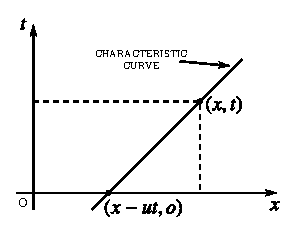
\includegraphics{figures/fig52-1.1.eps}
\caption{}\label{c1:fig1.1}
\end{figure}

\begin{exercise}\label{chap1:exer1.3}
Find\pageoriginale an analytic expression for $\rho (x,t)$ in terms
of $\rho (x,0)$ and $u(x,t)$ when $u$ is not longer constant.
\end{exercise}

\begin{remark}\label{chap1:rem1.3}
As such that advection equation is not difficult to solve
exactly. However when coupled with the other equations of fluid
dynamics difficulties arise and one looks for an efficient numerical
scheme of approximation. But one must be cautious in the choice of
such a scheme or else a ``diffusion process'' is likely to be
introduced into the approximate equation while no such thing exists in
the exact case. We will se this later.
\end{remark}

\section{The wave equations}\label{chap1:sec1.7}

We specialize to the case when $\mu = k=0$, and assume that $g$ is
negligible. Then L3 becomes
\begin{equation*}
\frac{D\varepsilon}{Dt} + p \frac{D}{Dt} \left(\frac{1}{\rho}\right) =
0. \tag{1.17} \label{eq1.17}
\end{equation*}
This together with the equation of state (Cf. (\ref{eq1.2})) can be integrated
to give a relationship between $p$ and $\rho$. For instance, in the
case of a perfect gas, we get $p \rho^{-\gamma} = \varphi(a)$,
$\varphi(a)$ being a constant if the initial state of the fluid is
constant. In this case the equations L1 and L2 read as 
\begin{equation*}
\left.
\begin{aligned}
& \frac{D\rho}{Dt} + \rho \frac{\partial u}{\partial x} = 0\\
& \frac{Du}{Dt} + \frac{1}{\rho} \frac{\partial}{\partial x}
(p(\rho)) =0.
\end{aligned} \right\}
\tag{1.18}\label{eq1.18}
\end{equation*}
Writing in vector form, we get
\begin{equation*}
\frac{D}{Dt} 
\begin{bmatrix}
\rho\\
u
\end{bmatrix} + 
\begin{bmatrix}
0 & \rho\\
\frac{p'(\rho)}{\rho} & 0
\end{bmatrix} \frac{\partial}{\partial x} 
\begin{bmatrix}
\rho\\
u
\end{bmatrix} =0
\tag{1.19}\label{eq1.19}
\end{equation*}

As such this equation is non-linear. If one wants to study small
perturbations\pageoriginale around a constant state of the fluid at
rest at time $t=0$, on e can linearize the state equation as 
\begin{equation*}
p - p_\circ = {C}^2_\circ (\rho - \rho_\circ) 
\tag{1.20}\label{eq1.20}
\end{equation*}
where $p_\circ, \rho_\circ , C_\circ$ are respectively the
pressure, density and sound-speed of the constant state at $t=0$. By
neglecting second order terms one can then write
\begin{equation*}
\frac{D}{Dt} \begin{bmatrix}
\rho\\u
\end{bmatrix} + 
\begin{bmatrix}
0 & \rho_\circ\\
C^2_\circ/ \rho_\circ & 0
\end{bmatrix} \frac{\partial}{\partial x} \begin{bmatrix}
\rho\\
u
\end{bmatrix} = 0.
\tag{1.21}\label{eq1.21}
\end{equation*}
Setting
\begin{align*}
\varphi & = \frac{\rho}{\rho_\circ} + \frac{u}{C_\circ}\\
\psi & = \frac{\rho}{\rho_\circ} - \frac{u}{C_\circ},
\end{align*}
we get, on substitution into (\ref{eq1.21}),
\begin{equation*}
\left.\begin{aligned}
 \frac{\partial \varphi}{\partial t} + C_\circ \frac{\partial
  \varphi}{\varphi x} & = 0\\
\frac{\partial \psi}{\partial t} - C_\circ \frac{\partial
  \psi}{\partial x} & = 0
\end{aligned}
\right\}
\tag{1.22}\label{eq1.22}
\end{equation*}
which are of the advective type. We know that $\varphi$, $\psi$ assume
the form
\begin{equation*}
\left.
\begin{aligned}
\varphi (x,t) & = \varphi (x-C_\circ t, 0)\\
\psi (x,t) & = \psi (x + C_\circ t, 0).
\end{aligned} \right\}
\tag{1.23}\label{eq1.23}
\end{equation*}

We now have two characteristic curves $x - C_\circ t =$ constant and
$x + C_\circ t = $ constant. The value at $(x,t)$ is now dependent on
the values over the {\em finite} interval $[ x -C_\circ t, x + C_\circ
t]$ on the real axis (Cf. Fig. \ref{c1:fig1.2}). 

\begin{figure}[H]
\centering
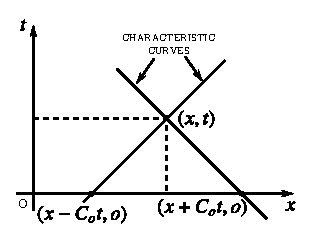
\includegraphics{figures/fig52-1.2.eps}
\caption{}\label{c1:fig1.2}
\end{figure}\pageoriginale

\section{The heat equation}\label{chap1:sec1.8}

We assume $\rho $ to be constant and $u$ to be zero. Then using an
equation of state like (\ref{eq1.3}), L3 will read as 
\begin{equation*}
\frac{\partial T}{\partial t} - \frac{\partial}{\partial x} \left(k
\frac{\partial T}{\partial x}\right) = 0. 
\tag{1.24}\label{eq1.24}
\end{equation*}
In particular if $k$ is a constant then we have
$$
T(x,t) = \frac{1}{2\sqrt{k\pi t}} \int\limits^{+\infty}_{-\infty} \exp
\left(\frac{-(x-y)^2}{4kt}\right)  T(y,0) dy.
$$ 

This shows that unlike the advective or the wave equations, the value
at $(x,t)$ of the solution of the heat equation depends on the initial
value, on the {\em entire} real line.

Our immediate aim is to study the mathematical properties of these
three types of equations and methods of approximating them.

\medskip
\noindent{\textbf{References:}}
General references for the entire course are Richtmyer and Morton
\cite{key32}, Potter \cite{key30}, Ames \cite{key2} and Mitchell
\cite{key27}. For the equations of fluid dynamics and their properties
one can refer to Courant and Friedrichs \cite{key9}. 

